\documentclass{article}
\usepackage{Sweave}
\begin{document}

\title{Online Appendix 2 for: Are divergence point analyses suitable for response time data?}
\author{Pablo Gomez, Javier Breithaupt, Manuel Perea, Jeff Rouder}

\Sconcordance{concordance:OnlineAppendix.tex:OnlineAppendix.Rnw:%
1 1 1 1 0 50 1}

\maketitle
\section{Abstract}

We applied the original divergence point method to simulated data. Our findings agree with Reingold \& Sheridan 2014. The outcome of this method is influenced by the number of trials. 


\section{Applying the method}


What happens when the divergence-point analysis is applied to a realistic example?  Well, the algorithm guarantees a real-valued answer so long as the distributions differ somewhere (and they do in the examples presented below).   In small sample sizes, the smaller differences at the bottom of the distribution cannot be detected and divergence points in the middle of the distribution might be expected.  But in larger sample sizes, the estimate will shift radically downward.  In the large sample limit, the estimate will shift downward without bound (at least theoretically, although in practice the divergence point is bounded by the shortest latencies).  

        As an illustration, we generated data from an ex-Gaussian distribution assuming that the experimental effect was either in the $\mu$ or $\tau$ parameters.  We manipulated the number of hypothetical trials per condition and then applied the bootstrapping method to estimate the divergence point.

      In the first simulation, we generated data in which the difference between the two conditions was an effect on $\mu$.  The data for the baseline condition was generated from an ex-Gaussian distribution with $\mu= 541$, $\sigma = 68$, and $\tau = 115$ . We generated data for three simulated experimental conditions by changing $\mu$ to 561, 581 and 621  ($\Delta \mu = 20, 40, 80$) There is, therefore, stochastic dominance of the baseline condition relatively to all of these other conditions, and the true divergence point is at the starting point of the distributions.  The results from this simulation are not encouraging for the method, as the estimation of the divergence point is highly biased by the number of trials per condition ($n = 20, 30, 50, 100, 250, 500, 1000$).   Figure 1 shows the average divergence point for each of the parameter combinations ($\mu$ and $n$) across 1000 simulations. As a consequence of increased statistical power due to larger sample size at the trial level, the larger the number of trials per condition, the shorter the estimated divergence point (i.e., there is a statistical bias dependent on sample size). For example, with $\Delta \mu =  80$, and $n=50$, the divergence point is about 100ms higher than for $n = 1000$.  In fact, when the number of trials is below 100, the different conditions are indistinguishable from each other. 
      
          
\begin{figure}[h] %  figure placement: here, top, bottom, or page
	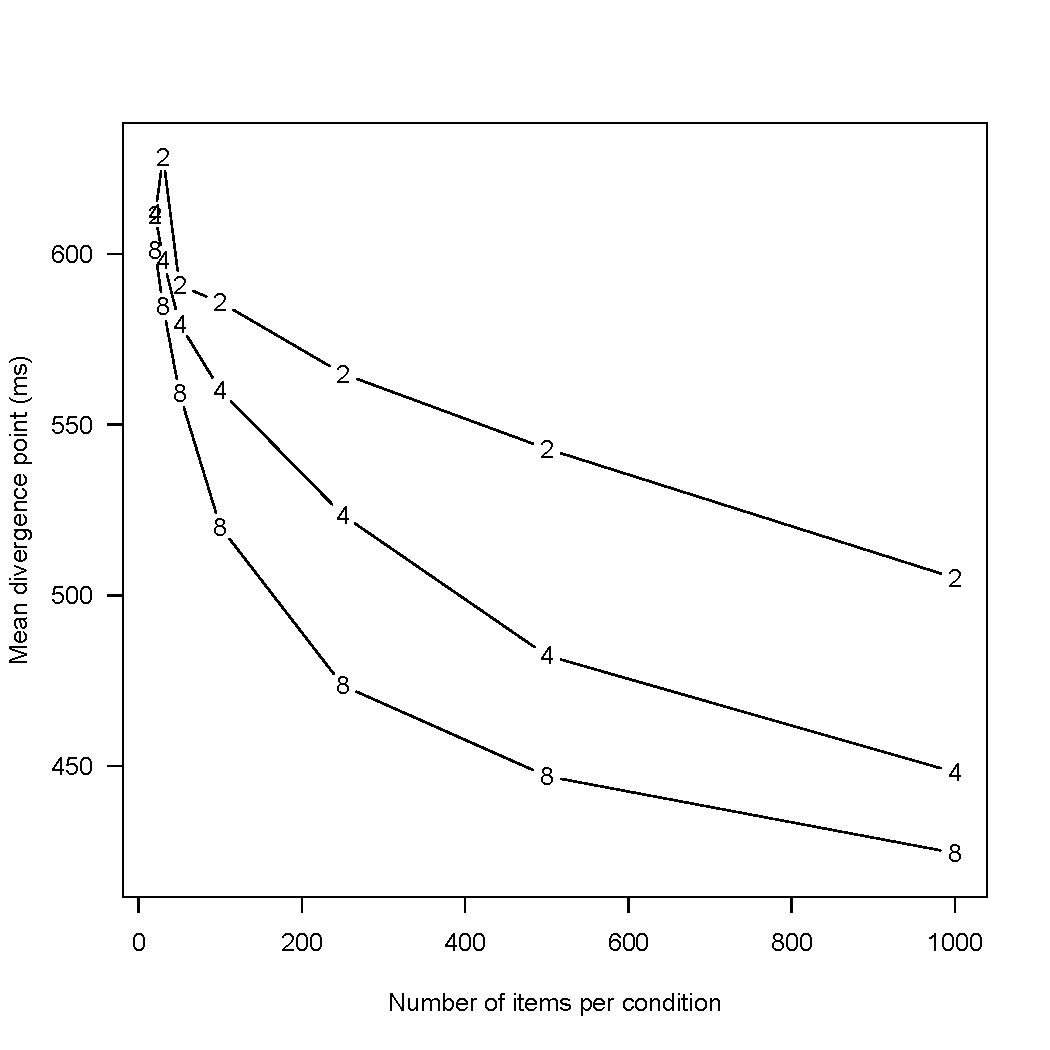
\includegraphics[width=5in]{Figure5.pdf}
	\caption{The figure shows average divergence point for simulated data using ex-Gaussian distributions with effects on $\mu$. The points represent the size of the effect in $\mu$ ($2$:20 ms; $4$: 40 ms; $8$: 80 ms).}
		\label{fig:mu-div}
\end{figure}
  
      In the second simulation, we generated latency data in which the difference between the two conditions was an effect on $\tau$.  The data for the baseline condition was the same as in the previous simulations: it was generated from an ex-Gaussian distribution with $\mu= 541$, $\sigma = 68$, and $\tau = 115$.  We generated data for three simulated experimental conditions by changing $\tau$ to 135, 155 and 195  ($\Delta \tau = 20, 40, 80$). As shown in Figure~2, changes in $\tau$  produce stochastic dominance of the baseline condition and the true divergence point is at the starting point of the distributions.   The results from this simulation are very similar to those from the first simulation: The estimation of the divergence point is severely biased by the number of trials per condition (n = 20, 30, 50, 100, 250 or 500).   Figure~2 shows the average divergence point for each of the parameter combinations ($\tau$ and $n$) across 1000 simulations.
   
\begin{figure}[h] %  figure placement: here, top, bottom, or page
	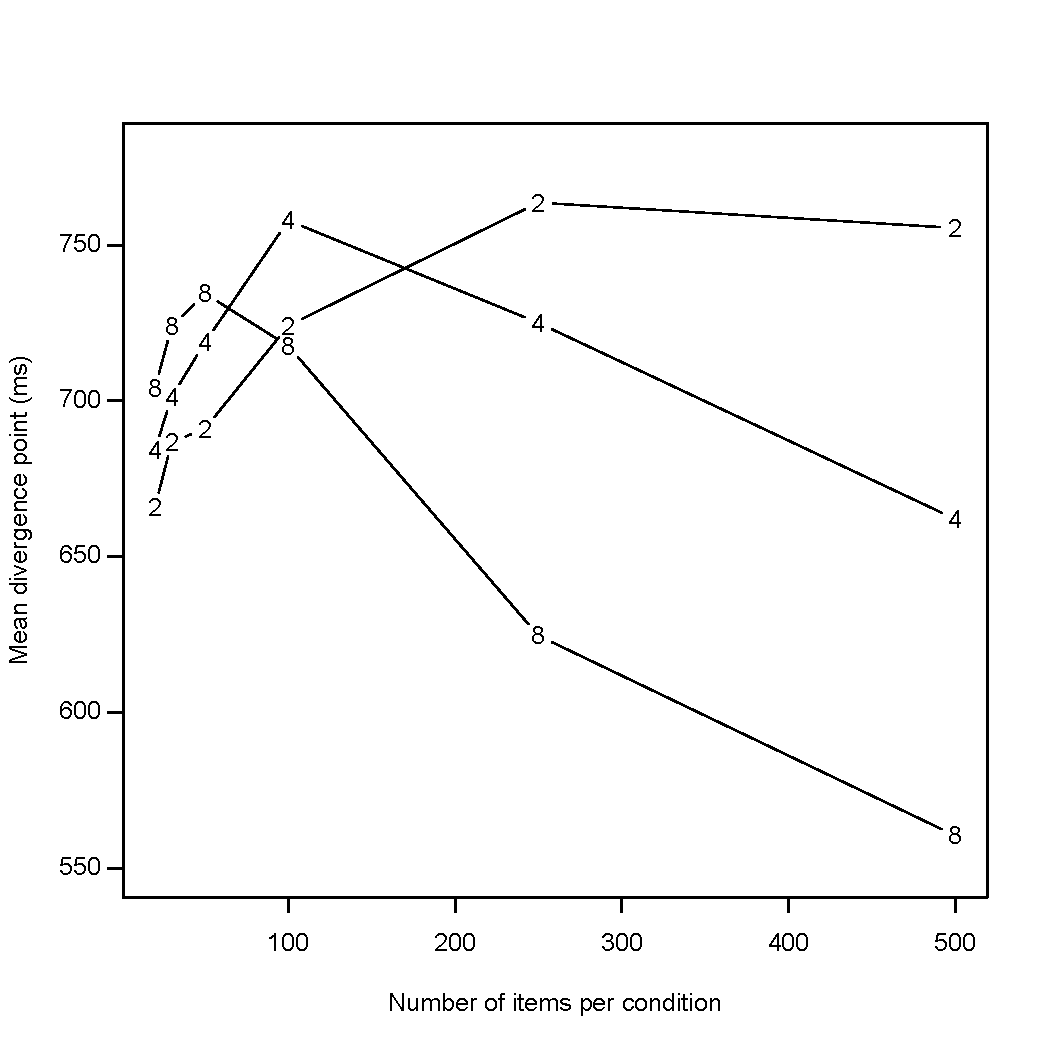
\includegraphics[width=5in]{Figure6.pdf}
	\caption{The figure shows average divergence point for simulated data using ex-Gaussian distributions with effects on $\tau$. The points represent the size of the effect in $\tau$ ($2$:20 ms; $4$: 40 ms; $8$: 80 ms).}
	\label{fig:tau-div}
\end{figure}


  
\section{Conclusion}

If the method is applied to data, an estimate of the divergence point will be provided by the method. This estimate will be affected mostly by the number of observations. Reingold \& Sheridan (2014) had alredy recognized this issue. They mentioned that `` ... divergence point would be delayed relative to the actual point of divergence. This would be especially the case under low experimental power (i.e., a small number of participants and observations)". They change the method to mitigate this issue, but given the nature of the method, the estimation of divergece point is necessarily biased (i.e., the average of  the sampling distribution of a estimated diverge point is not equal to the true divergence).

\newpage

\section{References}

Reingold, E. M., \& Sheridan, H. (2014). Estimating the divergence point: a novel distributional analysis procedure for determining the onset of the influence of experimental variables. \emph{Frontiers in Psychology, 5,} 1432. doi:10.3389/fpsyg.2014.01432



\end{document}
